
\chapter{Funzione \emph{main} del modulo sistema}
Con le spiegazioni precedenti abbiamo tutte le nozioni necessarie per approfondire le prime funzioni del modulo sistema eseguite dall'emulatore.
\section{Premessa: funzione \emph{start} (indirizzi moduli, IDT, costruttori, chiamata main)}
Prendiamo la funzione \emph{start} in \emph{sistema.s}, eseguita non appena il bootloader cede il controllo.
\small
\begin{verbatim}
	.globl  _start, start
	_start:				// entry point
	start:
	pushq %rdi
	
	// inizializziamo la IDT
	call init_idt
	
	// Il C++ prevede che si possa eseguire del codice prima di main (per
	// es. nei costruttori degli oggetti globali). gcc organizza questo
	// codice in una serie di funzioni di cui raccoglie i puntatori
	// nell'array __init_array_start. Il C++ run time deve poi chiamare
	// tutte queste funzioni prima di saltare a main.  Poiche' abbiamo
	// compilato il modulo con -nostdlib dobbiamo provvedere da soli a
	// chiamare queste funzioni, altrimenti gli oggetti globali non saranno
	// inizializzati correttamente.
	movabs $__init_array_start, %rbx
	1:	 cmpq $__init_array_end, %rbx
	je 2f
	call *(%rbx)
	addq $8, %rbx
	jmp 1b
	
	// il resto dell'inizializzazione e' scritto in C++
	2:	 popq %rdi
	call main
	// se arrivamo qui c'e' stato un errore, fermiamo la macchina
	hlt
\end{verbatim}
\normalsize 
%\begin{center}
%	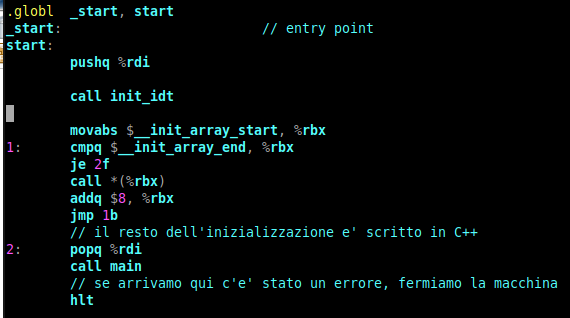
\includegraphics[scale=.9]{img/267.PNG}
%\end{center} 
\begin{enumerate}
	\item Pongo temporaneamente in pila il contenuto del registro RDI. Il contenuto consiste nel puntatore a una struttura \emph{multiboot$\_$info}, che contiene l'indirizzo dei moduli I/O e utente. 
	\item Chiamiamo \emph{init$\_$idt} per inizializzare la \emph{Interrupt Descriptor Table} (nei modi visti prima).
	\item Effettuo una serie di chiamate di costruttori relativi a oggetti globali.
	\item Recupero dalla pila il contenuto del registro RDI.
	\item Chiamata della funzione \emph{main}, scritta in C++ e contenente il resto dell'inizializzazione. Il codice della funzione è in \emph{sistema.cpp}. Si osservi che
	\begin{verbatim}
		extern "C" void main(paddr mbi) ...
	\end{verbatim}
	RDI è parametro di ingresso della funzione \emph{main}.
\end{enumerate}
\section{Primo processo, inizializzazione di GDT e APIC, associazione del tipo al piedino del timer}
Nelle prime righe:
\begin{itemize}
	\item definisco le caratteristiche del primo processo
	\begin{verbatim}
		// anche se il primo processo non è completamente inizializzato,
		// gli diamo un identificatore, in modo che compaia nei log
		init.id = 0xFFFF;
		init.precedenza = MAX_PRIORITY;
		init.cr3 = readCR3();
		esecuzione = &init;
	\end{verbatim}
	dove \emph{init} è un \emph{des$\_$proc} inizializzato nello stesso file
	\begin{verbatim}
		// un primo des_proc, allocato staticamente, da usare durante l'inizializzazione
		des_proc init;
	\end{verbatim}
	\item Chiamo \emph{init$\_$gdt} per inizializzare la \emph{Global Descriptor Table} (nei modi visti prima)
	\begin{verbatim}
		flog(LOG_INFO, "Nucleo di Calcolatori Elettronici, v6.5");
		init_gdt();
		flog(LOG_INFO, "GDT inizializzata");
	\end{verbatim}
	\item Inizializzo l'APIC e associo il tipo $2$ al piedino del timer.
	\begin{verbatim}
		apic_init(); // in libce
		apic_reset(); // in libce
		apic_set_VECT(2, TIPO_TIMER);
		flog(LOG_INFO, "APIC inizializzato");
	\end{verbatim}
\end{itemize}
\small

\normalsize 
\section{Inizializzazione di $M2$ e indirizzi virtuali dei vari intervalli}	
All'interno del codice si ha la chiamata della funzione \emph{init$\_$frame}, con cui inizializziamo $M2$. La parte $M1$ è già disponibile: è stata caricata dal \emph{bootloader} e contiene il modulo sistema.
\small 
\begin{verbatim}
	// inizializziamo la parte M2
	init_frame();
	flog(LOG_INFO, "Numero di frame: %d (M1) %d (M2)", N_M1, N_M2);
	
	flog(LOG_INFO, "sis/cond [%p, %p)", ini_sis_c, fin_sis_c);
	flog(LOG_INFO, "sis/priv [%p, %p)", ini_sis_p, fin_sis_p);
	flog(LOG_INFO, "io /cond [%p, %p)", ini_mio_c, fin_mio_c);
	flog(LOG_INFO, "usr/cond [%p, %p)", ini_utn_c, fin_utn_c);
	flog(LOG_INFO, "usr/priv [%p, %p)", ini_utn_p, fin_utn_p);
\end{verbatim}
\normalsize 
\subsection{Funzione \emph{init$\_$frame}}
La funzione \emph{init$\_$frame} si occupa di inizializzare i frame relativi alla parte di memoria non ancora utilizzata dopo il caricamento del modulo sistema: $M2$. 
\small 
\begin{verbatim}
	void init_frame() {
		// primo frame di M2
		paddr fine_M1 = allinea(reinterpret_cast<paddr>(&end), DIM_PAGINA);
		// numero di frame in M1 e indice di f in vdf
		N_M1 = fine_M1 / DIM_PAGINA;
		// numero di frame in M2
		N_M2 = N_FRAME - N_M1;
		
		if (!N_M2)
		return;
		
		// creiamo la lista dei frame liberi, che inizialmente contiene tutti i  frame di M2
		primo_frame_libero = N_M1;
		#ifndef N_STEP
		// alcuni esercizi definiscono N_STEP == 2 per creare mapping non
		// contigui in memoria virtale e controllare meglio alcuni possibili
		// bug
		#define N_STEP 1
		#endif
		for (natq i = N_M1; i < N_FRAME - N_STEP; i++) {
			vdf[i].prossimo_libero = i + N_STEP;
			num_frame_liberi++;
		}
		vdf[N_FRAME - N_STEP].prossimo_libero = 0;
	}
\end{verbatim}
\normalsize 
%\begin{center}
%	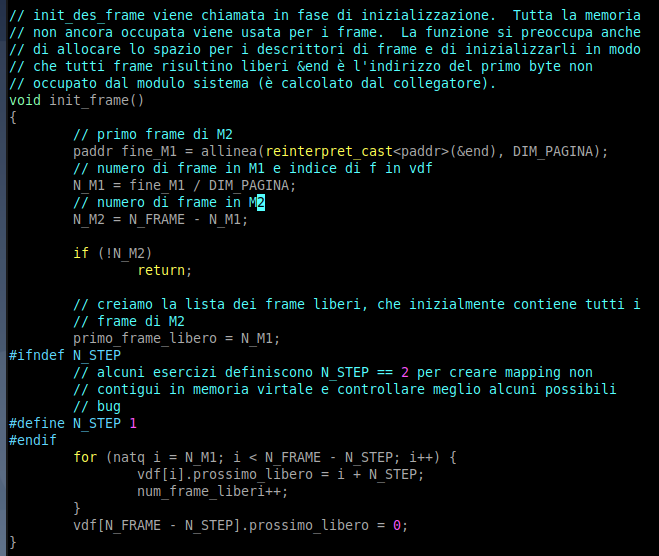
\includegraphics[scale=.8]{img/264.PNG}
%\end{center}  
\begin{itemize}
	\item \textbf{Cosa conosciamo?} 
	
	Si consideri la variabile \emph{end}, che contiene l'indirizzo del primo byte non occupato dal modulo sistema (calcolato dal collegatore). Conosciamo il numero di frame totali \emph{N$\_$FRAME}, calcolato dividendo la dimensione totale della memoria e la dimensione di ciascuna pagina.
	\item \textbf{Funzione \emph{allinea}}.
	
	Trovo il primo frame libero di $M2$ 
	\begin{verbatim}
		paddr fine_M1 = allinea(reinterpret_cast<paddr>(&end), DIM_PAGINA);
	\end{verbatim}
	utilizzando la funzione di utilità \emph{allinea}, che calcola il primo indirizzo multiplo di \emph{DIM$\_$PAGINA}  maggiore del primo argomento.
	\item A partire dal numero precedente otteniamo il numero di frame in $M1$ e quelli in $M2$
	\begin{verbatim}
		N_M1 = fine_M1 / DIM_PAGINA;
		N_M2 = N_FRAME - N_M1;
	\end{verbatim}
	\item Se non ci sono frame disponibili in $M2$ mi fermo subito.
	\begin{verbatim}
		if(!N_M2)
		return;
	\end{verbatim}
	\item Se ci sono frame creiamo la lista dei frame liberi attraverso un for: facciamo in modo che ogni descrittore di frame presente nel vettore \emph{vdf} punti al successivo. L'ultimo descrittore nel vettore non punta a niente, mentre il primo (la testa) viene puntato da \emph{primo$\_$frame$\_$libero}.
\end{itemize}
\subsection{Indirizzi virtuali iniziali e finali di tutti gli intervalli}
Nelle seguenti variabili, poste nella sezione dedicata alla paginazione di \emph{sistema.cpp}, andiamo a memorizzare degli indirizzi...
\small 
\begin{verbatim}
	// indirizzo virtuale di partenza delle varie zone della memoria virtuale dei processi
	const vaddr ini_sis_c = norm(I_SIS_C * dim_region(MAX_LIV - 1)); // sistema condivisa
	const vaddr ini_sis_p = norm(I_SIS_P * dim_region(MAX_LIV - 1)); // sistema privata
	const vaddr ini_mio_c = norm(I_MIO_C * dim_region(MAX_LIV - 1)); // modulo IO
	const vaddr ini_utn_c = norm(I_UTN_C * dim_region(MAX_LIV - 1)); // utente condivisa
	const vaddr ini_utn_p = norm(I_UTN_P * dim_region(MAX_LIV - 1)); // utente privata
	
	// indirizzo del primo byte che non appartiene alla zona specificata
	const vaddr fin_sis_c = ini_sis_c + dim_region(MAX_LIV - 1) * N_SIS_C;
	const vaddr fin_sis_p = ini_sis_p + dim_region(MAX_LIV - 1) * N_SIS_P;
	const vaddr fin_mio_c = ini_mio_c + dim_region(MAX_LIV - 1) * N_MIO_C;
	const vaddr fin_utn_c = ini_utn_c + dim_region(MAX_LIV - 1) * N_UTN_C;
	const vaddr fin_utn_p = ini_utn_p + dim_region(MAX_LIV - 1) * N_UTN_P;
\end{verbatim}
\normalsize 
%\begin{center}
%	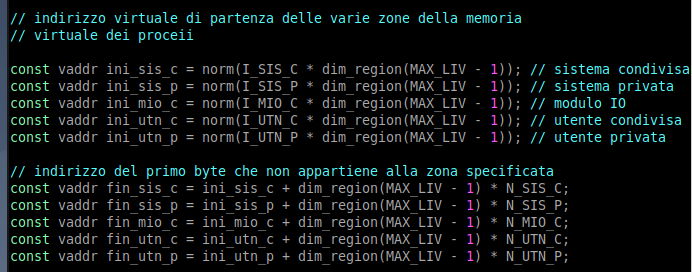
\includegraphics{img/257.PNG}
%\end{center}
\begin{itemize}
	\item Nel codice vengono calcolati gli indirizzi iniziali e finali di tutti gli intervalli definiti a inizio lezione. Sono tutti \emph{vaddr}.
	\item Per quanto riguarda le prime costanti devo trovare l'indirizzo di partenza dell'area.\\Moltiplico l'indice per la dimensione della regione di livello \emph{MAX$\_$LIV} - 1.
	\item Normalizzo con la funzione di utilità \emph{norm} per sistemare i bit più significativi.
\end{itemize}

\section{Allocazione di una tabella radice e creazione della finestra sulla memoria fisica}	
\small 
\begin{verbatim}
	// creiamo le parti condivise della memoria virtuale di tutti i processi
	// le parti sis/priv e usr/priv verranno create da crea_processo()
	// ogni volta che si attiva un nuovo processo
	paddr root_tab = alloca_tab();
	if (!root_tab)
	goto error;
	
	// finestra di memoria, che corrisponde alla parte sis/cond
	if(!crea_finestra_FM(root_tab))
	goto error;
\end{verbatim}
\normalsize 
%\begin{center}
%	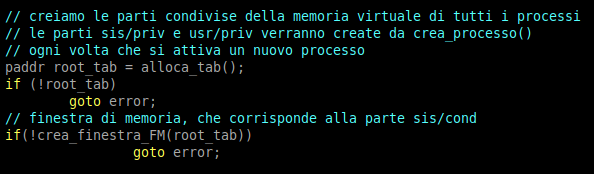
\includegraphics{img/271.PNG}
%\end{center}
\begin{itemize}
	\item Allochiamo una prima tabella radice con \emph{alloca$\_$tab}.
	\item Dobbiamo creare la finestra di memoria. In realtà il bootloader ne ha già creata una, ma non ci piace:
	\begin{itemize}
		\item è accessibile a livello utente;
		\item l'indirizzo $0$ è mappabile.
	\end{itemize}
	facciamo queste cose chiamando la funzione \emph{crea$\_$finestra$\_$fm}.
\end{itemize}
\subsection{Funzione \emph{crea$\_$finestra$\_$fm}}
La funzione \emph{crea$\_$finestra$\_$fm} crea la finestra che dicevamo prima. 
\small 
\begin{verbatim}
	bool crea_finestra_FM(paddr root_tab) {
		auto identity_map = [] (vaddr v) -> paddr { return v; };
		// mappiamo tutta la memoria fisica:
		// - a livello sistema (bit U/S non settato)
		// - scrivibile (bit R/W settato)
		// - con pagine di grandi dimensioni (bit PS)
		//   (usiamo pagine di livello 2 che sono sicuramente disponibili)
		
		// vogliamo saltare la prima pagina per intercettare *NULL, e inoltre
		// vogliamo settare per il bit PWT per la pagina che contiene la memoria
		// video.  Per farlo dobbiamo rinunciare a settare PS per la prima regione
		natq first_reg = dim_region(1);
		if (map(root_tab, DIM_PAGINA, first_reg, BIT_RW, identity_map) != first_reg)
		return false;
		
		// settiamo il bit PWT per la pagina che contiene la memoria video.
		// Usiamo un tab_iter su una sola pagina, fermandoci sul descrittore
		// "foglia" che contiene la traduzione.
		tab_iter it(root_tab, 0xb8000, DIM_PAGINA);
		while (it.down())
		;
		
		tab_entry& e = it.get_e();
		e |= BIT_PWT;
		
		// mappiamo il resto della memoria con PS settato
		if (MEM_TOT > first_reg) {
			if (map(root_tab, first_reg, MEM_TOT, BIT_RW, identity_map, 2) != MEM_TOT)
			return false;
		}
		
		flog(LOG_INFO, "Creata finestra sulla memoria centrale:  [%p, %p)", DIM_PAGINA, MEM_TOT);
		
		// Mappiamo gli ultimi 20MiB prima di 4GiB settando sia PWT che PCD.
		// Questa zona di indirizzi è utilizzata dall'APIC per mappare i propri registri.
		vaddr start_pci = 4*GiB - 20*MiB,
		end_pci = 4*GiB;
		if (map(root_tab, start_pci, end_pci, BIT_RW|BIT_PCD|BIT_PWT, identity_map, 2) != end_pci)
		return false;
		
		flog(LOG_INFO, "Creata finestra per memory-mapped-IO:    [%p, %p)", start_pci, end_pci);
		return true;
	}
\end{verbatim}
\normalsize 
\begin{framed}
	\noindent \textbf{Osservazione della funzione \emph{map}}. Osserviamo dall'uso della funzione \emph{map} che questa restituisce l'ultimo indirizzo mappato. Quando chiamiamo la funzione indichiamo un estremo finale: se la funzione restituisce l'estremo finale della finestra significa che tutto è andato bene, altrimenti qualcosa è andato storto. In alcuni casi (anche in prove d'esame) può essere necessario chiamare la funzione \emph{unmap}, per annullare il "mappaggio" fatto fino all'indirizzo restituito.
\end{framed} 
\begin{itemize}
	\item \textbf{Indirizzo $0$}.
	
	La prima pagina non viene mappata a causa dell'indirizzo $0$, che vogliamo disabilitare e usare per \emph{nullptr}. La cosa si risolve facilmente ignorando i primi indirizzi.
	\item \textbf{Pagina contenente la memoria video}.
	
	Usiamo \emph{map} nella tabella radice \emph{root$\_$tab}, a partire da DIM$\_$PAGINA fino alla fine della prima regione. Si pone il bit RW (ma non US) e la funzione \emph{identity$\_$map} (scritta con una notazione diversa dal solito) per restituire l'identità.
	\begin{verbatim}
		// vogliamo saltare la prima pagina per intercettare *NULL, e inoltre
		// vogliamo settare per il bit PWT per la pagina che contiene la memoria
		// video.  Per farlo dobbiamo rinunciare a settare PS per la prima regione
		natq first_reg = dim_region(1);
		if (map(root_tab, DIM_PAGINA, first_reg, BIT_RW, identity_map) != first_reg)
		return false;
	\end{verbatim}
	\textbf{Perchè mappiamo solo fino alla prima regione? }
	
	Vogliamo mettere il bit PWT  solo sulla memoria video (che sta in mezzo, dobbiamo lavorare su delle pagine in particolare). Lo facciamo utilizzando un iteratore.
	\begin{verbatim}
		// settiamo il bit PWT per la pagina che contiene la memoria video.
		// Usiamo un tab_iter su una sola pagina, fermandoci sul descrittore
		// "foglia" che contiene la traduzione.
		tab_iter it(root_tab, 0xb8000, DIM_PAGINA);
		while (it.down())
		;
		
		tab_entry& e = it.get_e();
		e |= BIT_PWT;
	\end{verbatim}
	Col while scorriamo l'albero arrivando a una foglia. Sappiamo che sicuramente la foglia avrà bit $P=1$ (abbiamo appena sistemato le traduzioni con la \emph{map}). Quando arriviamo alla foglia settiamo il flag con l'operatore OR. Non posso agire su aree di memorie molto specifiche, come in questo caso, se mappo gli indirizzi usando il \emph{Page Size Flag} (una traduzione mi identificherebbe un'area di memoria troppo grande).
	
	\item \textbf{Pagine rimanenti}. 
	
	A questo punto possiamo mappare il resto della memoria in un colpo solo, ricorrendo al \emph{Page Size Flag}.
	\begin{verbatim}
		// mappiamo il resto della memoria con PS settato
		if (MEM_TOT > first_reg) {
			if (map(root_tab, first_reg, MEM_TOT, BIT_RW, identity_map, 2) != MEM_TOT)
			return false;
		}
	\end{verbatim}
	
	\item \textbf{\emph{Memory-mapped I/O}}.
	
	Concludiamo mappando in memoria gli indirizzi relativi alle periferiche (\emph{Memory-mapped I/O}). In particolare è presente l'APIC, che utilizza indirizzi di memoria per i registri. 
	\small
	\begin{verbatim}
		// Mappiamo gli ultimi 20MiB prima di 4GiB settando sia PWT che PCD.
		// Questa zona di indirizzi è utilizzata dall'APIC per mappare i propri registri.
		vaddr start_pci = 4*GiB - 20*MiB,
		end_pci = 4*GiB;
		if (map(root_tab, start_pci, end_pci, BIT_RW|BIT_PCD|BIT_PWT, identity_map, 2) != end_pci)
		return false;
	\end{verbatim}
	\normalsize 
	Gli indirizzi si trovano negli ultimi $20\,\text{MiB}$, alla fine dei primi $4\,\text{GiB}$. Per il calcolo degli estremi utilizziamo le costanti \emph{GiB} e \emph{MiB}. Mettiamo tra i flag RW, PCD E PWT (la politica deve essere diversa per forza, in particolare è vitale disattivare la cache).
\end{itemize}
\paragraph{Osservazione da ricordare}
\[\boxed{\text{Non abbiamo usato il bit U/S. La finestra si usa solo con livello di privilegio sistema.}}\]
\clearpage 


\section{Creazione dello spazio condiviso}
\paragraph{Dove siamo arrivati} Con lo step precedente abbiamo creato la finestra, quindi lo spazio di indirizzamento virtuale necessario per lavorare a livello sistema. Adesso ci rimane da creare e mappare lo spazio rimanente, riservato a modulo I/O e modulo utente.
\paragraph{Codice}
\small 
\begin{verbatim}
	// parti io/cond e usr/cond, che contengono i segmenti ELF dei
	// moduli I/O e utente caricati dal boot loader
	if (!crea_spazio_condiviso(root_tab, mbi))
	goto error;
	
	flog(LOG_INFO, "Create le traduzioni per le parti condivise");
	flog(LOG_INFO, "Frame liberi: %d (M2)", num_frame_liberi);
\end{verbatim}
\normalsize 
%\begin{center}
%	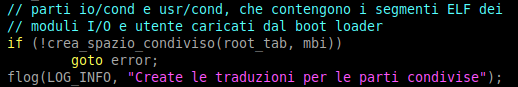
\includegraphics{img/276.PNG}
%\end{center}
Nel codice viene chiamata la funzione \emph{crea$\_$spazio$\_$condiviso}. Non approfondiremo fin troppo il contenuto (\textit{troppo complesso}, cit), ricordiamoci che:
\begin{itemize}
	\item il bootloader ci fornisce gli indirizzi di memoria fisica dove ha copiato i file relativi ai moduli (attraverso la struttura \emph{multiboot$\_$info}, è qua che utilizzeremo il contenuto del registro RDI);
	\item all'interno il codice relativo a un certo modulo è gestito con una funzione a parte, entrambe fanno ricorso alla funzione di utilità \emph{carica$\_$modulo} (funzione molto complicata, che \textbf{interpreta il file ELF});
	\item i segmenti posti nel file ELF vengono mappati utilizzando la solita funzione \emph{map};
	\item lo spazio destinato allo heap del modulo viene mappato sempre usando la \emph{map}. Ricordiamo che ci limitiamo a preparare uno spazio secondo la dimensione massima indicata con la costante \emph{heap$\_$size}: lo spazio effettivo cambia dinamicamente durante l'esecuzione. La funzione utilizzata per indicare la funzione è la \emph{alloca$\_$frame}: si scelgono i frame (non ci importa che siano consecutivi), ottenendo ogni volta il corrispondente indirizzo fisico. 
\end{itemize}
Dopo l'esecuzione della funzione avremo tutte le entrate dello spazio condiviso in \emph{root$\_$tab}. 

\section{Registro CR3}

Aggiorniamo il contenuto del registro CR3 ponendo l'indirizzo della \emph{root$\_$tab}
\begin{verbatim}
	loadCR3(root_tab);
	flog(LOG_INFO, "CR3 caricato")
\end{verbatim}
Da questo punto in poi utilizzeremo le nostre traduzioni, non più quelle create dal bootloader.

\clearpage 

\section{Inizializzazione dello \emph{heap}}
Inizializziamo lo heap chiamando l'apposita funzione
\small 
\begin{verbatim}
	// Assegna allo heap di sistema HEAP_SIZE byte nel secondo MiB
	heap_init((void*)HEAP_START, HEAP_SIZE);
	flog(LOG_INFO, "Heap di sistema: %x B @%x", HEAP_SIZE, HEAP_START);
\end{verbatim}
\normalsize 
Si consideri la presenza delle seguenti funzioni, nel modulo sistema, per gestire lo \emph{heap}
\begin{verbatim}
	void* operator new(size_t size) {
		return alloca(size);
	}
	
	void* operator new(size_t size, align_val_t align) {
		return alloc_aligned(size, align);
	}
	
	void operator delete(void *p) {
		dealloca(p);
	}
\end{verbatim}
\section{Creazione processo sistema}
Creiamo un nuovo processo che lanceremo dopo aver concluso con la funzione \emph{main}.
\begin{verbatim}
	// creazione del processo main_sistema
	mid = crea_main_sistema(mbi);
	if (mid == 0xFFFFFFFF)
	goto error;
	flog(LOG_INFO, "Creato il processo main_sistema (id = %d)", mid);
\end{verbatim}
Il codice della funzione è il seguente:
\begin{verbatim}
	natl crea_main_sistema(natq mbi) {
		des_proc* m = crea_processo(main_sistema, mbi, MAX_PRIORITY, LIV_SISTEMA, false);
		if (m == 0) {
			flog(LOG_ERR, "Impossibile creare il processo main_sistema");
			return 0xFFFFFFFF;
		}
		inserimento_lista(pronti, m);
		processi++;
		return m->id;
	}
\end{verbatim}
\begin{itemize}
	\item Per prima cosa si usa la \emph{crea$\_$processo} per creare effettivamente il processo. 
	\begin{itemize}
		\item La funzione associata al processo è la \emph{main$\_$sistema}. Il suo unico parametro di ingresso è {mbi} (registro RDI, indirizzo al \emph{multiboot$\_$info}).
		\item La priorità è massima: \emph{MAX$\_$PRIORITY}.
		\item Il processo è eseguito con livello di privilegio sistema.
	\end{itemize}
	\item Dopo aver creato il processo lo pongo nella lista \emph{pronti}: avendo posto priorità massima finirà sicuramente in testa.
	\item Incremento il numero di processi creati.
	\item Concludo restituendo l'ID del processo creato.
\end{itemize}

\subsection{Funzione \emph{crea$\_$processo}, inizializzazione della pila sistema ed eventualmente della pila utente, inizializzazione del \emph{punt$\_$nucleo}}
Ogni volta che viene creato un processo chiamiamo la \emph{crea$\_$processo} (anche nella primitiva \emph{activate$\_$p}): indichiamo funzione, parametri, priorità, livello di privilegio, se le interruzioni sono attive o disattivate.
\begin{itemize}
	\item \textbf{Creazione del \emph{des$\_$proc}}.
	
	Alloco e resetto un \emph{des$\_$proc}, e ne riempio i campi.
	\small
	\begin{verbatim}
		// allocazione (e azzeramento preventivo) di un des_proc
		p = new des_proc;
		if (!p)
		goto errore1;
		memset(p, 0, sizeof(des_proc));
		
		// rimpiamo i campi di cui conosciamo già  i valori
		p->precedenza = prio;
		p->puntatore = nullptr;
		// il registro RDI deve contenere il parametro da passare alla funzione f
		p->contesto[I_RDI] = a;
	\end{verbatim}
	\normalsize
	\item \textbf{Ricerca di un identificatore per il processo}.
	
	Viene allocato un identificatore numerico, se non esiste più finiamo subito.
	\small
	\begin{verbatim}
		// selezione di un identificatore
		p->id = alloca_proc_id(p);
		if (p->id == 0xFFFFFFFF)
		goto errore2;
	\end{verbatim}
	\normalsize 
	dove \emph{alloca$\_$proc$\_$id} è una funzione di utilità
	\small
	\begin{verbatim}
		// alloca un id non utilizzato.
		natl alloca_proc_id(des_proc *p) {
			static natl next = 0;
			
			// La funzione inizia la ricerca partendo  dall'id successivo
			// all'ultimo restituito (salvato nella variable statica 'next'),
			// saltando quelli che risultano in uso.
			natl scan = next, found = 0xFFFFFFFF;
			do {
				if (proc_table[scan] == nullptr) {
					found = scan;
					proc_table[found] = p;
				}
				scan = (scan + 1) % MAX_PROC;
			} while (found == 0xFFFFFFFF && scan != next);
			next = scan;
			return found;
		}
	\end{verbatim}
	\normalsize 
	Scorro l'array finchè non individuo un'entrata non utilizzata. Se individuo un'entrata disponibile ne restituisco l'indice, altrimenti restituisco 0xFFFFFFFF.
	
	\item \textbf{Creazione della tabella per il \emph{trie}}.
	
	Creo una tabella che fungerà da radice del trie. 
	\begin{verbatim}
		// creazione della tabella radice del processo
		p->cr3 = alloca_tab();
		if (p->cr3 == 0)
		goto errore3;
		init_root_tab(p->cr3);
	\end{verbatim}
	Con la funzione \emph{init$\_$root$\_$tab} inizializzo il \emph{trie}. 
	\small
	\begin{verbatim}
		// inizializza la tabella radice di un nuovo processo
		void init_root_tab(paddr dest){
			paddr pdir = readCR3();
			
			copy_des(pdir, dest, I_SIS_C, N_SIS_C);
			copy_des(pdir, dest, I_MIO_C, N_MIO_C);
			copy_des(pdir, dest, I_UTN_C, N_UTN_C);
		}
	\end{verbatim}
	\normalsize
	\begin{itemize}
		\item La funzione ha in ingresso un paddr \emph{dest}, che consiste nel CR3 del contesto.
		\item Per prima cosa si pone in \emph{pdir} il contenuto del registro CR3, recuperando così l'indirizzo dell'attuale \emph{trie}.
		\item Copio dall'attuale \emph{trie} le traduzioni relative alle parti condivise: modulo sistema, modulo utente e modulo I/O. Il risultato sono alberi di processi diversi che presentano sottoalberi comuni: la cosa permette di risparmiare memoria.
	\end{itemize}
	\item \textbf{Creazione della pila sistema e funzione \emph{crea$\_$pila}}.
	
	L'unica cosa che ci manca da fare è creare la pila sistema.
	\small 
	\begin{verbatim}
		// creazione della pila sistema
		if (!crea_pila(p->cr3, fin_sis_p, DIM_SYS_STACK, LIV_SISTEMA))
		goto errore4;
	\end{verbatim}
	\normalsize 
	Lo facciamo con la funzione  \emph{crea$\_$pila}.
	\small
	\begin{verbatim}
		// crea una pila processo (utente o sistema, in base a 'liv').  Creiamo una
		// traduzione dagli indirizzi riservati alla pila verso frame allocati sul
		// momento.
		bool crea_pila(paddr root_tab, vaddr bottom, natq size, natl liv) {
			vaddr v = map(root_tab,
			bottom - size,
			bottom,
			BIT_RW | (liv == LIV_UTENTE ? BIT_US : 0),
			[](vaddr) { return alloca_frame(); }
			);
			if (v != bottom) {
				unmap(root_tab, bottom - size, v, [](vaddr p, int) { rilascia_frame(p); });
				return false;
			}
			return true;
		}
	\end{verbatim}
	\normalsize 
	\begin{itemize}
		\item Creiamo una pila nel \emph{trie} relativo al processo, utilizzando la funzione \emph{map}. Come funzione per indicare gli indirizzi utilizziamo, anche qua, la \emph{alloca$\_$frame}.
		\item Se la \emph{map} è fallita dobbiamo fare l'\emph{unamp} di quanto fatto dalla \emph{map} (possiamo farlo, abbiamo posto nella variabile \emph{v} l'ultimo indirizzo mappato). Le tabelle vengono distrutte, ovviamente, ciò che è vuoto. Per rilasciare i vari frame utilizza la \emph{rilascia$\_$frame}.
	\end{itemize}
	
	\item \textbf{Ottenimento dell'indirizzo fisico della pila}.
	\small 
	\begin{verbatim}
		pila_sistema = trasforma(p->cr3, fin_sis_p - DIM_PAGINA) + DIM_PAGINA;
	\end{verbatim}
	\normalsize 
	Gli indirizzi virtuali adottati per la pila sistema sono gli stessi in ogni processo, la cosa che cambia è il significato (la traduzione) attribuita all'indirizzo virtuale stesso. Il fatto è che se noi utilizziamo l'indirizzo senza porci troppi pensieri andiamo a manipolare l'albero del processo corrente, e non l'albero del processo che stiamo creando. Risolviamo la cosa utilizzando la funzione \emph{trasforma}.
	\small
	\begin{verbatim}
		// restituisce l'indirizzo fisico che corrisponde a ind_virt nell'albero
		// di traduzione con radice root_tab.
		paddr trasforma(paddr root_tab, vaddr v) {
			// usiamo un tab_iter su una sola pagina fermandoci sul
			// descrittore foglia lungo il percorso di traduzione di 'v'
			tab_iter it(root_tab, v);
			while (it.down())
			;
			
			// si noti che il percorso potrebbe essere incompleto.
			// Ce ne accorgiamo perchè il descrittore foglia ha il bit P a
			// zero. In quel caso restituiamo 0, che per noi non è un
			// indirizzo fisico valido.
			tab_entry e = it.get_e();
			if (!(e & BIT_P))
			return 0;
			
			// se il percorso è completo calcoliamo la traduzione corrispondente.
			// Si noti che non siamo necessariamente arrivati al livello 1, se
			// c'era un bit PS settato lungo il percorso.
			int l = it.get_l();
			natq mask = dim_region(l - 1) - 1;
			return (e & ~mask) | (v & mask);
		}
	\end{verbatim}
	\normalsize
	\begin{itemize}
		\item Si pone in ingresso l'indirizzo della radice del \emph{trie}, \emph{root$\_$tab}, e l'indirizzo virtuale \emph{v} (l'indirizzo che vogliamo tradurre).
		\item Si scorre l'albero usando l'iteratore \emph{tab$\_$iter} (stesso percorso della MMU, ma fatto in software). Arrivati alla foglia si verifica il valore del bit $P$:
		\begin{itemize}
			\item se è uguale a $0$ la traduzione non è valida e si restituisce 0;
			\item altrimenti la traduzione è valida e restituiamo l'indirizzo fisico.
		\end{itemize} 
		\item Attenzione alle somme e differenze presenti
		\begin{verbatim}
			pila_sistema = trasforma(p->cr3, fin_sis_p - DIM_PAGINA) + DIM_PAGINA\end{verbatim}
		Attenzione alla somma e alla differenza: voglio il \textit{bottom fisico} della pila, se io non faccio la differenza ottengo l'indirizzo del frame successivo (ricordarsi l'indirizzo puntato sulla pila quando non c'è niente).
	\end{itemize}
	
	\item \textbf{Contenuto della pila sistema}. 
	
	La pila sistema viene creata in un qualunque processo, come già spiegato dobbiamo riempirla. Il contenuto differisce lievemente in base al livello di privilegio 
	\small
	\begin{verbatim}
		// ----- PROCESSO DI LIVELLO UTENTE -----
		pl[-5] = reinterpret_cast<natq>(f); // RIP (codice utente)
		pl[-4] = SEL_CODICE_UTENTE;	    // CS (codice utente)
		pl[-3] = IF ? BIT_IF : 0;	    // RFLAGS
		pl[-2] = fin_utn_p - sizeof(natq);  // RSP
		pl[-1] = SEL_DATI_UTENTE;	    // SS (pila utente)
		// eseguendo una IRET da questa situazione, il processo
		// passera' ad eseguire la prima istruzione della funzione f,
		// usando come pila la pila utente (al suo indirizzo virtuale)
		
		// ----- PROCESSO DI LIVELLO SISTEMA -----
		pl[-6] = reinterpret_cast<natq>(f);  	// RIP (codice sistema)
		pl[-5] = SEL_CODICE_SISTEMA;            // CS (codice sistema)
		pl[-4] = IF ? BIT_IF : 0;  	        // RFLAGS
		pl[-3] = fin_sis_p - sizeof(natq);      // RSP
		pl[-2] = 0;			        // SS
		pl[-1] = 0;			        // ind. rit. (non significativo)
		// i processi esterni lavorano esclusivamente a livello
		// sistema. Per questo motivo, prepariamo una sola pila (la
		// pila sistema)
	\end{verbatim}
	\normalsize 
	
	\item \textbf{Eventuale creazione della pila utente}.
	
	Se il processo è di livello utente allora dobbiamo creare la relativa pila utente. La cosa non è invece necessaria se il processo è di livello sistema. 
	\small
	\begin{verbatim}
		// creazione della pila utente
		if (!crea_pila(p->cr3, fin_utn_p, DIM_USR_STACK, LIV_UTENTE)) {
			flog(LOG_WARN, "creazione pila utente fallita");
			goto errore5;
		}
	\end{verbatim}
	\normalsize 
	Anche in questo caso usiamo la funzione \emph{crea$\_$pila}. 
	\item \textbf{Inizializzazione di RSP}. 
	
	Un processo di livello utente si trova, inizialmente, a livello sistema (come se avessi eseguito un'istruzione INT): aggiorniamo RSP nel \emph{contesto}, in modo tale che punti all'ultimo elemento della pila sistema.
	\small 
	\begin{verbatim}
		// inizialmente, il processo si trova a livello sistema, come
		// se avesse eseguito una istruzione INT, con la pila sistema
		// che contiene le 5 parole lunghe preparate precedentemente
		p->contesto[I_RSP] = fin_sis_p - 5 * sizeof(natq);
	\end{verbatim}
	\normalsize 
	L'inizializzazione di RSP si fa anche con un processo di livello sistema, ma ponendo in pila anche l'indirizzo di ritorno (che però non è significativo)
	\small 
	\begin{verbatim}
		// inizializziamo il descrittore di processo
		p->contesto[I_RSP] = fin_sis_p - 6 * sizeof(natq);
	\end{verbatim}
	\normalsize 
	
	\item \textbf{Inizializzazione del \emph{punt$\_$nucleo}}.
	
	Se stiamo gestendo un processo di livello utente dobbiamo inizializzare \emph{punt$\_$nucleo} (in un processo di livello sistema non è necessario, avremo solo la pila sistema)
	\small
	\begin{verbatim}
		// dal momento che usiamo traduzioni diverse per le parti sistema/private
		// di tutti i processi, possiamo inizializzare p->punt_nucleo con un
		// indirizzo (virtuale) uguale per tutti i processi
		p->punt_nucleo = fin_sis_p;
	\end{verbatim}
	\normalsize  L'indirizzo posto verrà copiato in TSS, in modo che il meccanismo delle interruzioni utilizzi questo indirizzo per il cambio pila. 
	
	\textbf{Fermi tutti}: se abbiamo un unico indirizzo virtuale potremo evitare ogni volta la modifica dell'indirizzo nel TSS, basta solo cambiarne l'interpretazione nella traduzione usata dalla MMU.
	
\end{itemize}

\section{Creazione processo dummy}
Prima di passare la parola al processo creato con la \emph {crea$\_$main$\_$sistema} dobbiamo creare il processo dummy con la funzione \emph{crea$\_$dummy} (ricordare le motivazioni per cui lo facciamo).
\small 
\begin{verbatim}
	// creazione del processo dummy
	dummy_id = crea_dummy();
	if (dummy_id == 0xFFFFFFFF)
	goto error;
	flog(LOG_INFO, "Creato il processo dummy (id = %d)", dummy_id);
\end{verbatim}
\normalsize 
\section{Schedulatore}
Chiamiamo lo schedulatore
\begin{verbatim}
	schedulatore();
\end{verbatim}
La funzione pone nel puntatore \emph{esecuzione} il processo creato in \emph{crea$\_$main$\_$sistema} (a cui abbiamo dato massima priorità, troveremo in testa per forza quello).


\section{Funzione \emph{salta$\_$a$\_$main}}
Il codice della funzione si conclude con la chiamata della funzione \emph{salta$\_$a$\_$main}.
\small 
\begin{verbatim}
	// esegue CALL carica_stato; IRETQ (vedi "sistema.s"). Il resto
	// dell'inizializzazione prosegue più comodamente nel processo
	// main_sistema(), che può essere interrotto e può sospendersi.
	salta_a_main();
\end{verbatim}
\normalsize
La sua implementazione è in \emph{sistema.s}
\small
\begin{verbatim}
	.global salta_a_main
	salta_a_main:
	call carica_stato
	iretq
\end{verbatim}
\normalsize
Con la \emph{carica$\_$stato} e la \emph{iretq} avviene il passaggio al processo creato con la \emph{crea$\_$main$\_$sistema}, con cui viene eseguita (a livello sistema) la funzione \emph{main$\_$sistema}.

\section{Funzione \emph{main$\_$sistema}}
Concludiamo con la funzione \emph{main$\_$sistema}, ultimo step prima del primo processo utente.
\small 
\begin{verbatim}
	void (*io_entry)(natq);
	void (*user_entry)(natq);
	
	void main_sistema(natq mbi) {
		natl sync_io;
		natl id;
		
		// occupiamo a_p[2] (in modo che non possa essere sovrascritta
		// per errore tramite activate_pe()) e smascheriamo il piedino
		// 2 dell'APIC
		a_p[2] = ESTERN_BUSY;
		apic_set_MIRQ(2, false);
		// attiviamo il timer, in modo che i processi di inizializzazione
		// possano usare anche delay(), se ne hanno bisogno.
		attiva_timer(DELAY);
		flog(LOG_INFO, "Timer attivato (DELAY=%d)", DELAY);
		
		// inizializzazione del modulo di io
		// Creiamo un processo che esegua la procedura cmain del modulo I/O.
		// Usiamo un semaforo di sincronizzazione per sapere quando
		// l'inizializzazione è terminata.
		sync_io = sem_ini(0);
		if (sync_io == 0xFFFFFFFF) {
			flog(LOG_ERR, "Impossibile allocare il semaforo di sincr per l'IO");
			goto error;
		}
		id = activate_p(io_entry, sync_io, MAX_PRIORITY, LIV_SISTEMA);
		if (id == 0xFFFFFFFF) {
			flog(LOG_ERR, "impossibile creare il processo main I/O");
			goto error;
		}
		flog(LOG_INFO, "Creato il processo main I/O (id = %d)", id);
		flog(LOG_INFO, "attendo inizializzazione modulo I/O...");
		sem_wait(sync_io);
		flog(LOG_INFO, "... inizializzazione modulo I/O terminata");
		
		// creazione del processo start_utente
		id = activate_p(user_entry, 0, MAX_PRIORITY, LIV_UTENTE);
		if (id == 0xFFFFFFFF) {
			flog(LOG_ERR, "impossibile creare il processo main utente");
			goto error;
		}
		flog(LOG_INFO, "Creato il processo start_utente (id = %d)", id);
		
		// terminazione
		flog(LOG_INFO, "passo il controllo al processo utente...");
		terminate_p();
		
		error: panic("Errore di inizializzazione");
	}
\end{verbatim}
\normalsize 
\begin{itemize}
	\item Attenzione all'array \emph{a$\_$p} (andiamo a fare l'assegnamento per evitare confusione con la funzione per l'attivazione dei processi esterni, che vedremo più avanti). Con la \emph{apic$\_$set$\_$MIRQ} attiviamo l'ascolto delle interruzioni sul piedino. Attiviamo il timer con la funzione \emph{attiva$\_$timer}: ricordarsi che l'implementazione del timer stesso è posta nel modulo sistema e non nel modulo I/O (per permettere l'implementazione, ad esempio, della funzione \emph{delay}).
	\item Creo il semaforo \emph{sync$\_$io}, creo un processo con funzione quella puntata da \emph{io$\_$entry} e passo come parametro l'identificativo del semaforo. Questa cosa permetterà di eseguire le inizializzazioni del modulo I/O, affrontate nel capitolo del codice del Modulo I/O.
	\small
	\begin{verbatim}
		sync_io = sem_ini(0);
		[...]
		id = activate_p(io_entry, sync_io, MAX_PRIORITY, LIV_SISTEMA);
		[...]
		flog(LOG_INFO, "Creato il processo main I/O (id = %d)", id);
		flog(LOG_INFO, "attendo inizializzazione modulo I/O...");
		sem_wait(sync_io);
		flog(LOG_INFO, "... inizializzazione modulo I/O terminata");
	\end{verbatim}
	\normalsize
	In particolare si osservi che non ritorneremo su questo codice finchè non verrà rilasciato il gettone \emph{sync$\_$io}. Questa cosa avviene nella funzione \emph{main} del Modulo I/O, dopo aver fatto le inizializzazioni necessarie (si  veda il felativo capitolo per approfondire).
	\item Creo il primo processo utente e termino l'attuale processo.
	\small 
	\begin{verbatim}
		// creazione del processo start_utente
		id = activate_p(user_entry, 0, MAX_PRIORITY, LIV_UTENTE);
		[...]
		flog(LOG_INFO, "Creato il processo start_utente (id = %d)", id);
		// terminazione
		flog(LOG_INFO, "passo il controllo al processo utente...");
		terminate_p();
	\end{verbatim}
	\normalsize
\end{itemize}